\section{Kevätjuhlassa ansioituneet}

\begin{figure}[!b]
\centering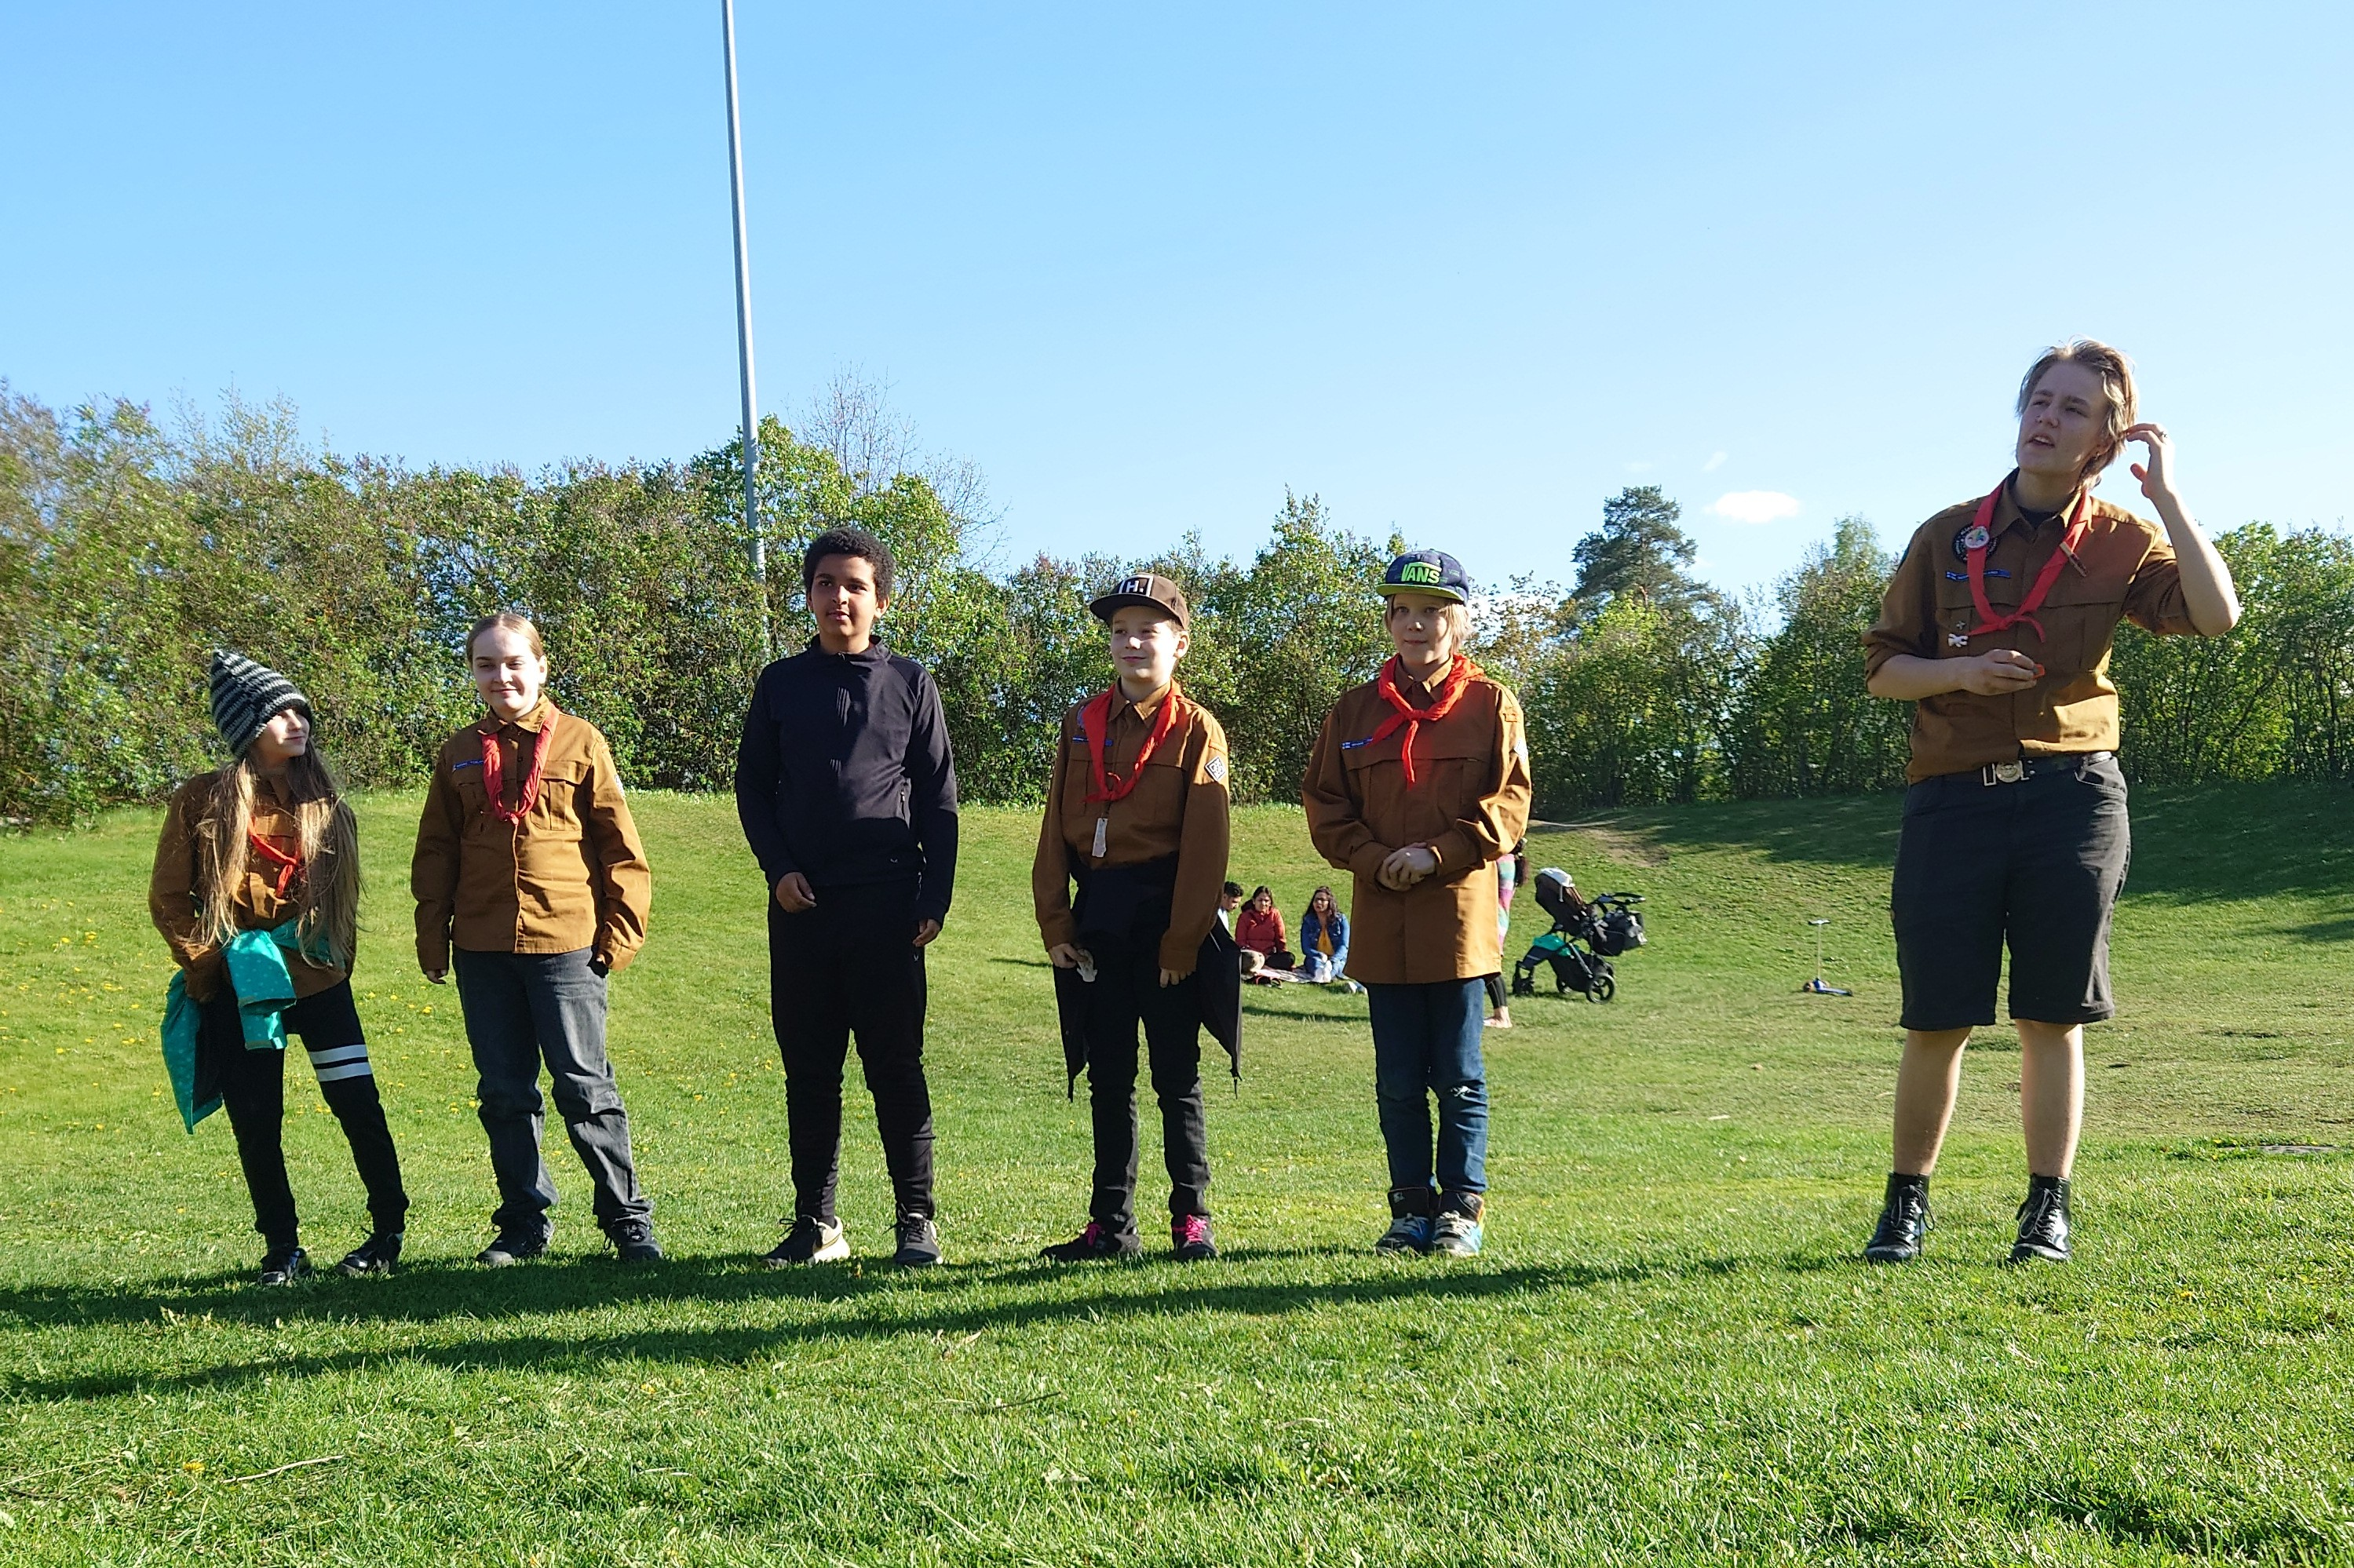
\includegraphics[width=\textwidth]{assets/kevatjuhla}
\end{figure}

\begin{multicols}{2}
\noindent Lippukunnan kevätjuhla järjestettiin perinteikkäästi leikkipuisto Kipinäpuistossa jo tutussa ''amfiteatterissa''. Juhlassa jaettiin parven ja vartioiden keväällä suorittamia merkkejä sekä annettiin partiolupaus.

Partiolupaus (seikkailijoihin siirtyvät): Eino, Linnea ja Vanamo.

Partiolupaus (vaeltajiin siirtyvät): Ahti, Elias, Leo ja Mikael. 

Ilmastosankari- ja liikunta"-jäljet: \textit{Kurjet}"-parvi (Alisa, Eino, Haley, Janja, Jella, Johannes, Lily, Linnea, Nella, Sade ja Vanamo).

Länsi"-ilmansuunta: \textit{Pomppupallot}"-vartio (Elna, Joella, Kuisma, Samuel ja Touko).

Yhteiskunta"-tarppo: \textit{Päärynähyttyset}"-vartio (Alden, Jetro, Ninni, Tesla ja Toivo).

Punainen nahkalilja: Alden, Elias ja Toivo.

Harmaa nahkalilja: Ahti, Leo ja Mikko.

Aktiivisimman kolkan kiertopalkinto: Alisa.

Kiitos"-pinssi: Kata, Leo ja Mikko.
\end{multicols}

\medskip

\noindent\null\hfill Kuva ja Teksti: Janne 
